\section{Проектирование физической модели телекоммуникационной системы организации}
\label{sec:3}
На основании разработанной структурной схемы организации создана физическая модель кабельной системы. При организации кабельной системы для сетей на основе проводных соединений должны учитываться различные факторы. При выборе кабеля в первую очередь учитывается требуемая длина, а также защищенность от помех и уровень собственных излучений. 

В состав торгового склада входят 2 здания: торговое и складское. Торговое здание является одноэтажным. Включает в себя 5 комнат: 3 торговых, 1 бухгалтерская и 1 серверная. Периметр здания \hyp{} 120м, площадь \hyp{} 800 $\text{м}^2$. Высота потолков \hyp{} 4 м, внешние стены кирпичные, внутренние перегородки и отделка гипсокартоновые. План торгового здания приведен на рисунке \ref{fig:shop-plane}.
\begin{figure}[H]
  \centering
  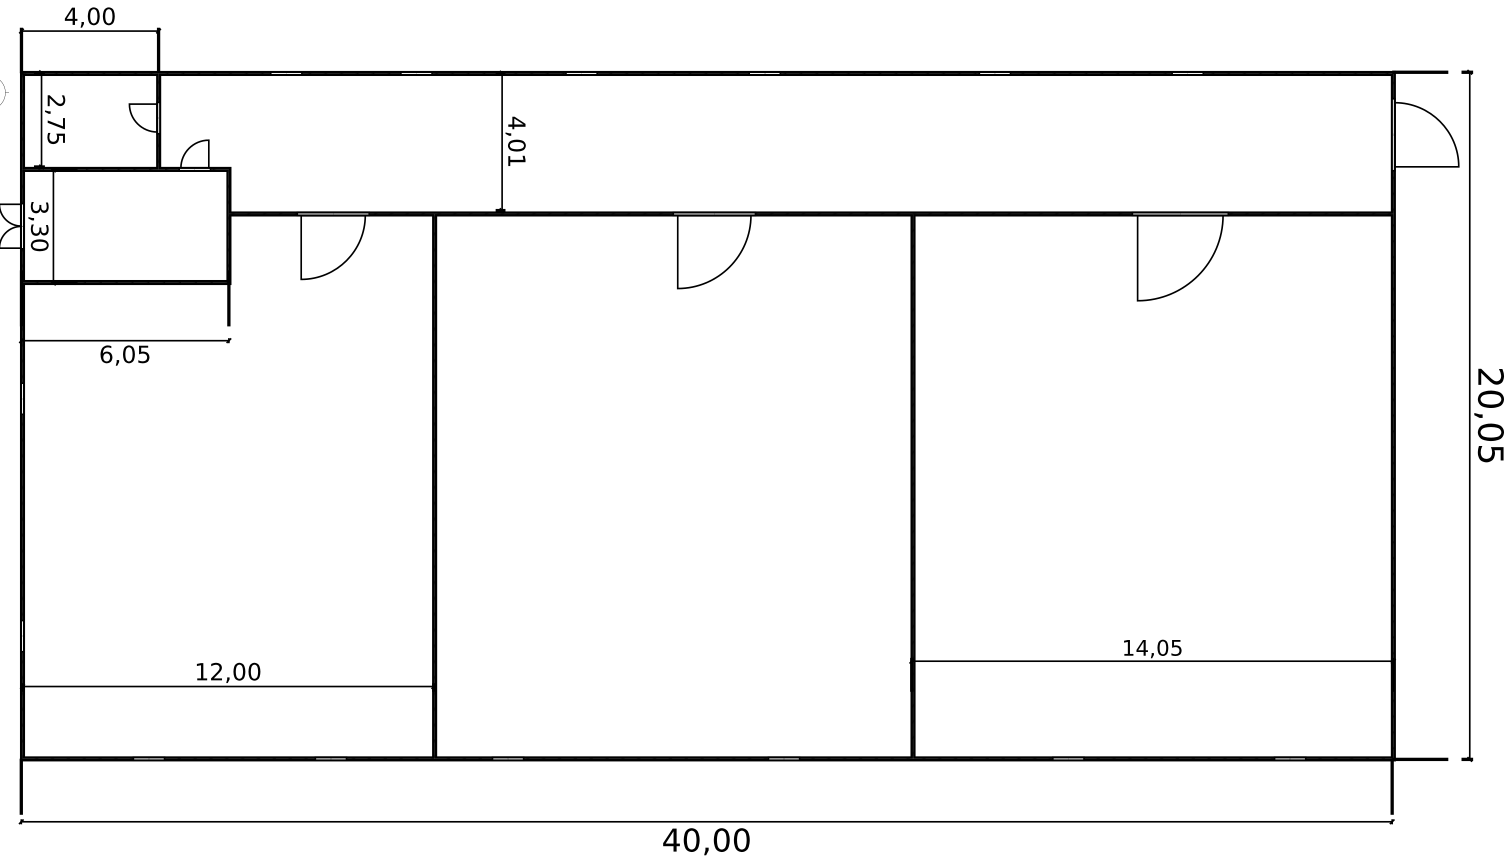
\includegraphics[width=\linewidth]{sec3/img/shop-plane.png}
  \caption{План торгового здания}
  \label{fig:shop-plane}
\end{figure}


Складское здание является одноэтажным. Включает в себя 3 складских помещения. Периметр здания 100 м, площадь \hyp{} 600 $\text{м}^2$. Высота потолков \hyp{} 6м, стены кирпичные, внутренняя отделка отсутствует. План складского здания приведен на рисунке \ref{fig:store-plane}.
\begin{figure}[H]
  \centering
  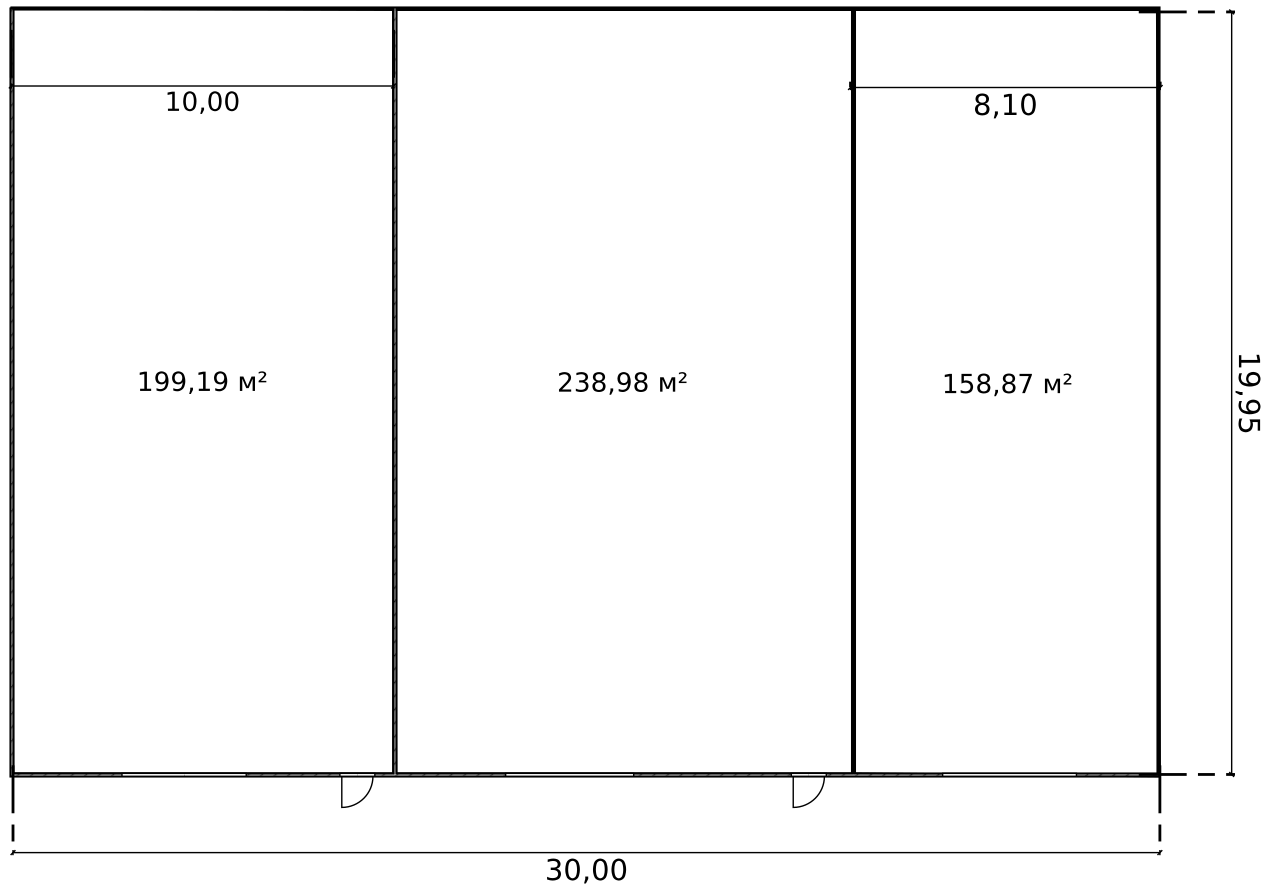
\includegraphics[width=\linewidth]{sec3/img/store-plane.png}
  \caption{План складского здания}
  \label{fig:store-plane}
\end{figure}

На планы зданий нанесено примерное расположение информационных розеток и АРМ. Результат выполнения для торгового и складского зданий приведен на рисунках \ref{fig:shop-arm} и \ref{fig:store-arm}.
\begin{figure}[H]
  \centering
  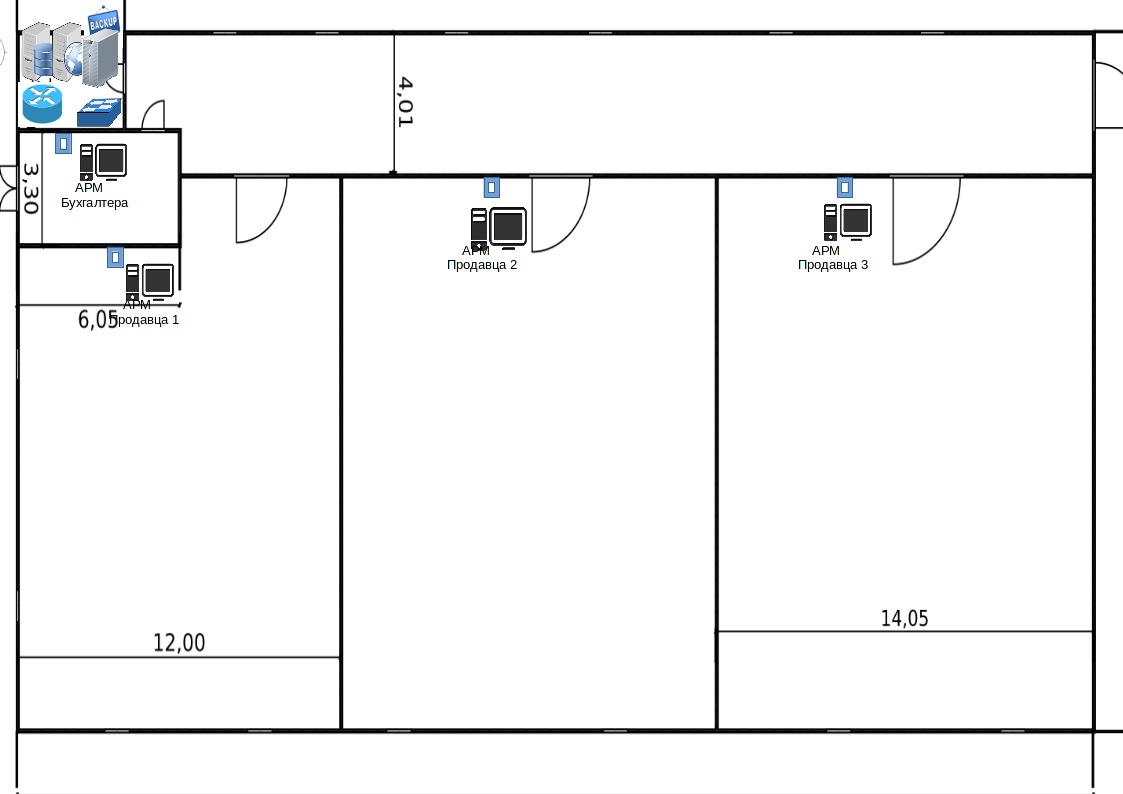
\includegraphics[width=\linewidth]{sec3/img/shop.png}
  \caption{План торгового здания с указанными положениями розеток и АРМ}
  \label{fig:shop-arm}
\end{figure}

\begin{figure}[H]
  \centering
  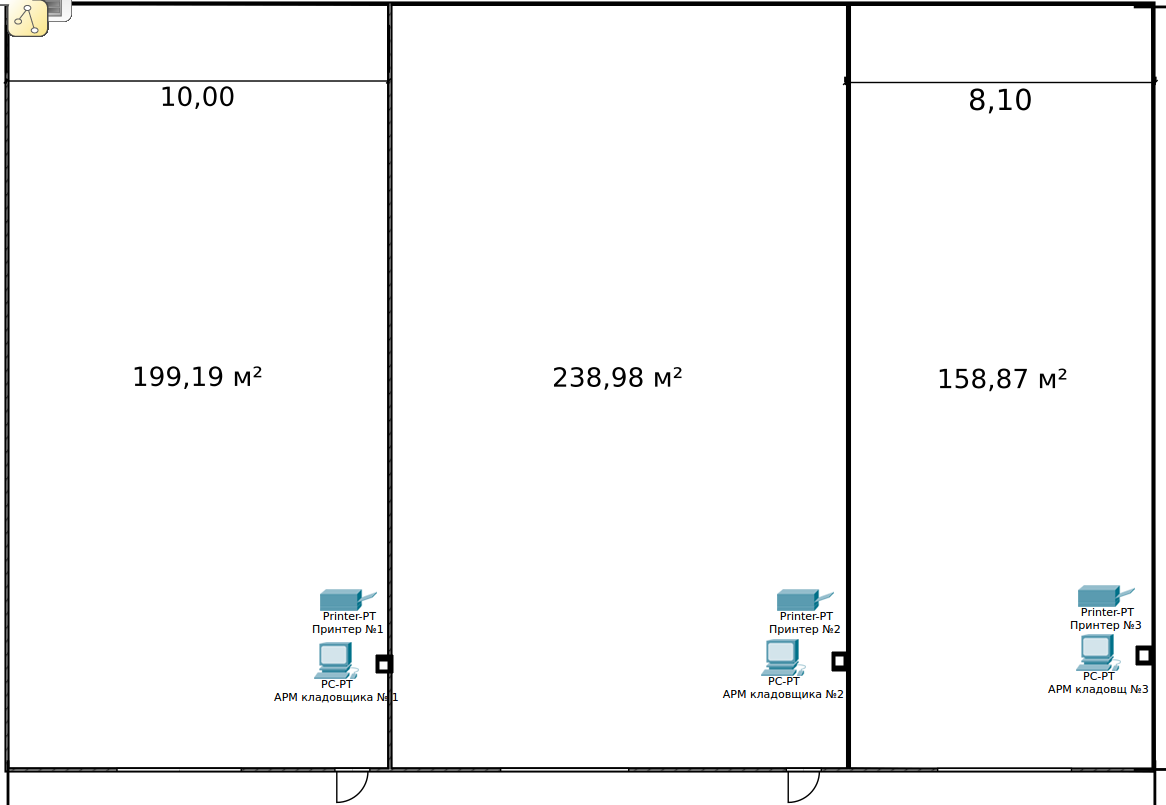
\includegraphics[width=\linewidth]{sec3/img/store.png}
  \caption{План складского здания с указанными положениями розеток и АРМ}
  \label{fig:store-arm}
\end{figure}

Сервера располaгаются в аппаратной комнате торгового здания, там же расположен телекоммуникационный шкаф, в котором размещаются коммутатор продавцов и роутер. Коммутатор кладовщиков расположен в первом помещении. Кабельная система проложена по внутренним стенам помещений на высоте 3 м от пола. Кабель, ведущий от складского до торгового здания, проложен под землей на глубине 0.5м. Расчетные длины кабелей приведены в таблице \ref{tab:cablen}.

\begin{table}[H]
  \centering
  \caption{Расчетные длины кабелей}
  \begin{tabular}{|l|l||l|l|} \hline
    Ресурс & Кабель, м & Ресурс & Кабель, м \\ \hline
    Сервер БД & 2м & АРМ продавца 1 & 1м\\ \hline
    Сервер Веб & 2м & АРМ продавца 2 & 1м \\ \hline
    Сервер бэкап & 2м & АРМ продавца 3 & 1м \\ \hline
    АРМ бухгалтера & 1м & АРМ кладовщ 1 & 1м \\ \hline
    АРМ кладовщ 3 & 1м & Принтер кладовщ 1 & 1м \\ \hline
    Принтер кладовщ 2 & 1м &АРМ кладовщ 2 & 1м \\ \hline
    Принтер кладовщ 3 & 1м& Принтер бухгалтера & 1м \\ \hline
  \end{tabular}
  \label{tab:cablen}
\end{table}

В каждом помещении имеется одна информационная розетка с двумя портами 8P8C. Розетки подключены с помощью 4-парного кабеля пятой категории (по 2 пары на порт), и прикреплены к стенам на высоте 30 см от пола.

В разрабатываемой ТКС предусмотрено 2 коммутатора. Первый коммутатор расположен в серверной торгового здания, а второй \hyp{} в помещении №1 склада. Прикреплены к стенам на высоте 3 метров. Конструкция торгового здания позволяет проводить кабель от розеток до коммутатора в стенах и потолке (т.к. перегородки гипсовые, а потолок подвесной). В складе кабели прикреплены к стенам пластиковыми хомутами. Расположение коммутаторов, роутера и прочего оборудования приведено на рисунках \ref{fig:shop-arm} и \ref{fig:store-arm}. Расчетные длины кабелей от розеток до коммутаторов приведены в таблице \ref{tab:crosscablen}

\begin{table}[H]
  \centering
  \caption{Расчетные длины кабелей от розеток до кроссового оборудования}
  \begin{tabular}{|l|l||l|l|} \hline
    Ресурс & Кабель, м & Ресурс & Кабель, м \\ \hline
    АРМ продавца1 & 8.5 & АРМ Кладовщ 1 & 5.7\\ \hline
    АРМ продавца2 & 12.7 & АРМ Кладовщ 2 & 28.7\\ \hline
    АРМ продавца3 & 25.7 & АРМ Кладовщ 3 & 35.5\\ \hline
    АРМ бухгалтера & 3.2 & & \\ \hline
  \end{tabular}
  \label{tab:crosscablen}
\end{table}

Разработанная физическая модель кабельной подсистемы локальной телекоммуникационной системы для торгового и складского зданий приведена на рисунках \ref{fig:cisco-shop} и \ref{fig:cisco-store} соответственно.

\begin{figure}[H]
  \centering
  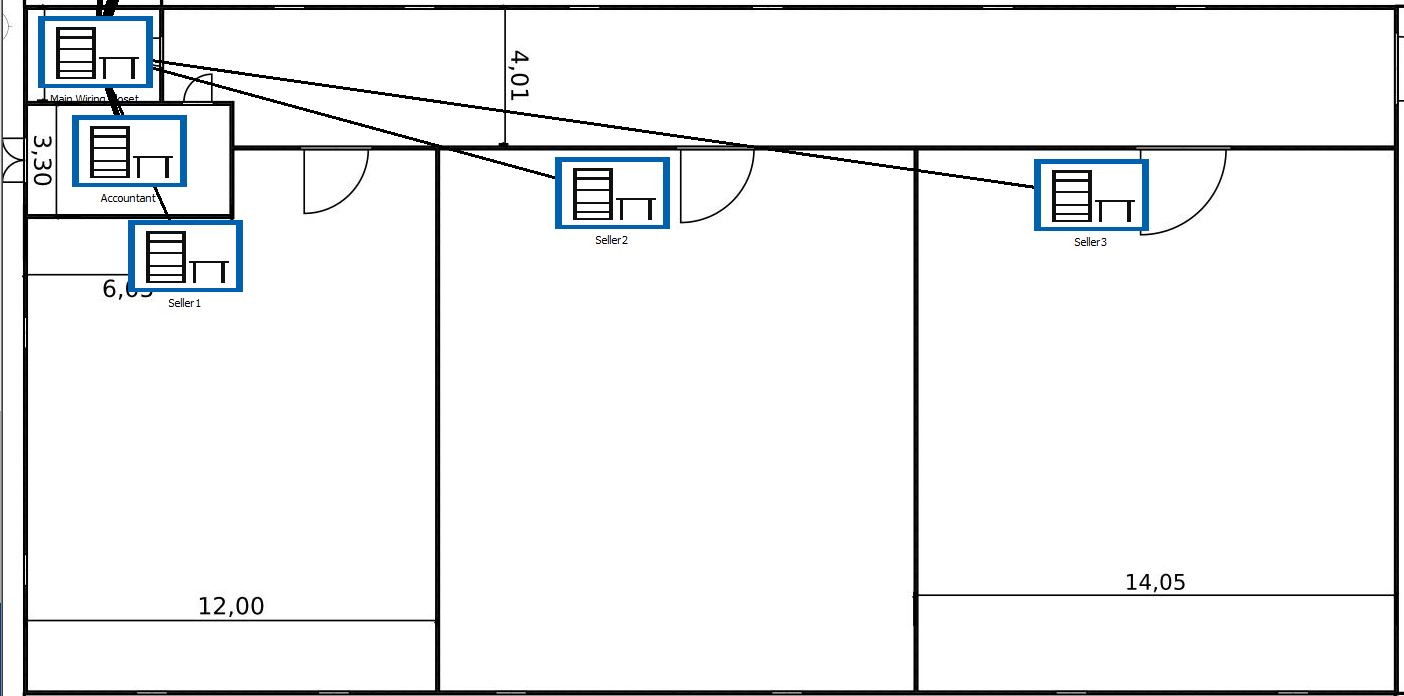
\includegraphics[width=\linewidth]{sec3/img/cisco-shop.png}
  \caption{Физическая модель кабельной подсистемы торгового здания}
  \label{fig:cisco-shop}
\end{figure}

\begin{figure}[H]
  \centering
  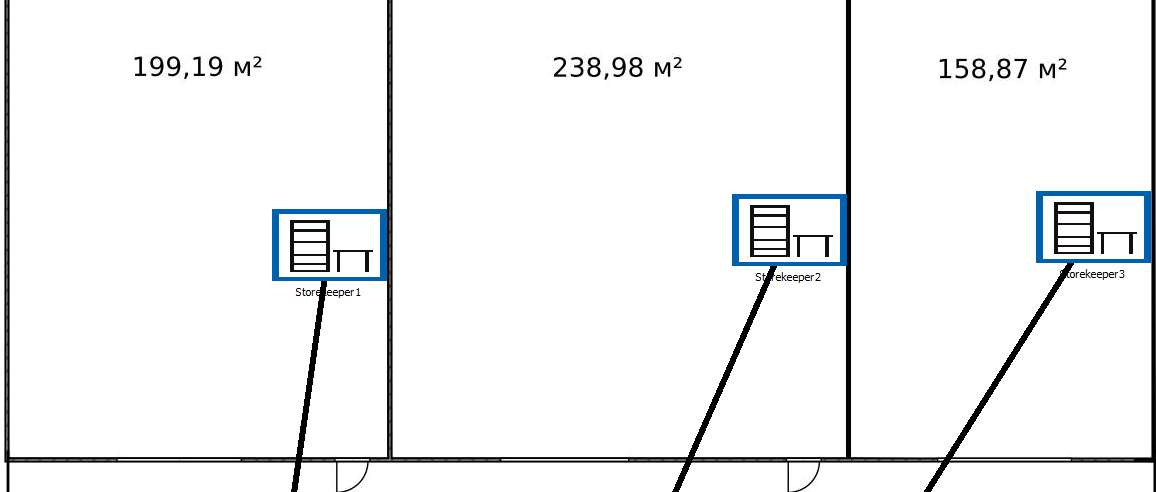
\includegraphics[width=\linewidth]{sec3/img/cisco-store.png}
  \caption{Физическая модель кабельной подсистемы складского здания}
  \label{fig:cisco-store}
\end{figure}


Для подключения к сети интернет необходим роутер с возможностью подключения оптоволоконных кабелей. Роутер, через который осуществляется подключение к интернету, расположен серверной комнате торгового здания.